
% This file was converted to LaTeX by Writer2LaTeX ver. 1.4
% see http://writer2latex.sourceforge.net for more info
%\documentclass[a4paper]{article}
%\usepackage[ascii]{inputenc}
%\usepackage[T1]{fontenc}
%\usepackage[english,spanish]{babel}
%\usepackage{amsmath}
%\usepackage{amssymb,amsfonts,textcomp}
%\usepackage{color}
%\usepackage{array}
%\usepackage{hhline}
%\usepackage{hyperref}
%\usepackage{pdfpages}

%\usepackage{xcolor}

\hypersetup{pdftex, colorlinks=true, linkcolor=black, citecolor=blue, filecolor=blue, urlcolor=blue, pdftitle=DOCUMENTO DE DISE\~NO DE VIDEOJUEGO, pdfauthor=Alex Verd\'u, pdfsubject=Da Vinci startup, pdfkeywords=}
% Outline numbering
\setcounter{secnumdepth}{0}
% List styles
\newcounter{saveenum}
\newcommand\liststyleLFOxii{%
\renewcommand\theenumi{\arabic{enumi}}
\renewcommand\theenumii{\alph{enumii}}
\renewcommand\theenumiii{\roman{enumiii}}
\renewcommand\theenumiv{\arabic{enumiv}}
\renewcommand\labelenumi{\theenumi.}
\renewcommand\labelenumii{\theenumii.}
\renewcommand\labelenumiii{\theenumiii.}
\renewcommand\labelenumiv{\theenumiv.}
}
\newcommand\liststyleLFOxi{%
\renewcommand\labelitemi{{\textbullet}}
\renewcommand\labelitemii{o}
\renewcommand\labelitemiii{${\blacksquare}$}
\renewcommand\labelitemiv{{\textbullet}}
}
\newcommand\liststyleLFOvi{%
\renewcommand\theenumi{\arabic{enumi}}
\renewcommand\theenumii{\alph{enumii}}
\renewcommand\theenumiii{\roman{enumiii}}
\renewcommand\theenumiv{\arabic{enumiv}}
\renewcommand\labelenumi{\theenumi.}
\renewcommand\labelenumii{\theenumii.}
\renewcommand\labelenumiii{\theenumiii.}
\renewcommand\labelenumiv{\theenumiv.}
}
\newcommand\liststyleLFOvii{%
\renewcommand\theenumi{\arabic{enumi}}
\renewcommand\theenumii{\alph{enumii}}
\renewcommand\theenumiii{\roman{enumiii}}
\renewcommand\theenumiv{\arabic{enumiv}}
\renewcommand\labelenumi{\theenumi.}
\renewcommand\labelenumii{\theenumii.}
\renewcommand\labelenumiii{\theenumiii.}
\renewcommand\labelenumiv{\theenumiv.}
}
\newcommand\liststyleLFOxiii{%
\renewcommand\labelitemi{{\textbullet}}
\renewcommand\labelitemii{o}
\renewcommand\labelitemiii{${\blacksquare}$}
\renewcommand\labelitemiv{{\textbullet}}
}
\newcommand\liststyleLFOxiv{%
\renewcommand\labelitemi{{\textbullet}}
\renewcommand\labelitemii{o}
\renewcommand\labelitemiii{${\blacksquare}$}
\renewcommand\labelitemiv{{\textbullet}}
}
% Page layout (geometry)
\setlength\voffset{-1in}
\setlength\hoffset{-1in}
\setlength\topmargin{0.984in}
\setlength\oddsidemargin{1.1812in}
\setlength\textheight{9.724999in}
\setlength\textwidth{5.9055996in}
\setlength\footskip{0.0cm}
\setlength\headheight{0cm}
\setlength\headsep{0cm}
% Footnote rule
\setlength{\skip\footins}{1.1777999mm}
\renewcommand\footnoterule{\vspace*{-0.007in}\setlength\leftskip{0pt}\setlength\rightskip{0pt plus 1fil}\noindent\textcolor{black}{\rule{0.33\columnwidth}{0.007in}}\vspace*{1mm}}
% Pages styles
\makeatletter
\newcommand\ps@MP{
  \renewcommand\@oddhead{}
  \renewcommand\@evenhead{}
  \renewcommand\@oddfoot{}
  \renewcommand\@evenfoot{}
  \renewcommand\thepage{\arabic{page}}
}
\newcommand\ps@MPF{
  \renewcommand\@oddhead{}
  \renewcommand\@evenhead{}
  \renewcommand\@oddfoot{}
  \renewcommand\@evenfoot{}
  \renewcommand\thepage{\arabic{page}}
}
\makeatother
\pagestyle{MP}
\title{DOCUMENTO DE DISE\~NO DE VIDEOJUEGO}
\author{Alex Verd\'u}
\date{2017-06-07}
%\begin{document}
\chapter{Anexo I. Documento de diseño de videojuego}
\label{GDD}

%
\includepdf[pages={1},pagecommand={},fitpaper=true,trim=0 0 0 0, 
%offset=0 0,turn=true,noautoscale=true]{anexos/GDD/portadaGDDImagen.pdf}


\clearpage\clearpage\setcounter{page}{1}\pagestyle{MP}
\thispagestyle{MPF}

\clearpage
\bigskip

\section[]{\selectlanguage{spanish} }
\section[Visi\'on general]{\selectlanguage{spanish} Visi\'on general}
\hypertarget{Toc484614208}{}\subsection[Introducci\'on]{\selectlanguage{spanish} Introducci\'on}
\hypertarget{Toc484614209}{}{\selectlanguage{spanish}
Este juego recrea una aventura ficticia del famoso inventor Leonardo da Vinci.\ }

{\selectlanguage{spanish}
A lo largo del juego,\ el inventor\ deber\'a desarrollar un producto, obtener financiaci\'on y venderlo siguiendo la
metodolog\'ia Lean Startup. Para ello contar\'a con los consejos de Andrea del\ Verrocchio que ser\'a su mentor en el
mundo del emprendimiento y las startups.}

{\selectlanguage{spanish}
El juego ser\'a una aventura gr\'afica al estilo del m\'itico juego Monkey island, aunque se desarrollar\'a en un
escenario 2.5D como en el t\'itulo Deadlight.}

\subsection[Tema]{\selectlanguage{spanish} Tema}
\hypertarget{Toc484614210}{}{\selectlanguage{spanish}
El juego se desarrolla en la Florencia\ renacentista, \'epoca en la que Leonardo trabaj\'o en el taller de Andrea de
Verrocchio. A lo largo de la partida se visitar\'an diversos escenarios como el taller de Andrea, las calles de
Florencia o los palacios de los burgueses.}

\subsection[Estilo visual]{\selectlanguage{spanish} Estilo visual}
\hypertarget{Toc484614211}{}{\selectlanguage{spanish}
Se utilizar\'an modelos 3D y texturas fotorealistas. No es necesario un gran nivel de detalle y/o de realismo pero se
evitar\'a una apariencia de estilo cartoon, comic o cel shading.}

\subsection[Influencias]{\selectlanguage{spanish} Influencias}
\hypertarget{Toc484614212}{}\subsubsection[Monkey island]{\selectlanguage{spanish} Monkey island}
\hypertarget{Toc484614213}{}{\selectlanguage{spanish}
Monkey island es uno de los referentes en cuanto a aventuras gr\'aficas se refiere.\ Da Vinci startup est\'a inspirado
en este juego y utiliza gran parte de sus mec\'anicas. Por ejemplo los di\'alogos interactivos en formato \'arbol, en
los que las decisiones tomadas por el jugador condicionan las respuestas de los personajes del juego.}

\subsubsection[Deadlight]{\selectlanguage{spanish} Deadlight}
\hypertarget{Toc484614214}{}{\selectlanguage{spanish}
Este juego (ver fig. \ref{deadlightImage}) posee un estilo similar al deseado en Da Vinci startup: un entorno 3D en el que el jugador se mueve en un
plano 2D.}

\begin{figure}
    \begin{center}
    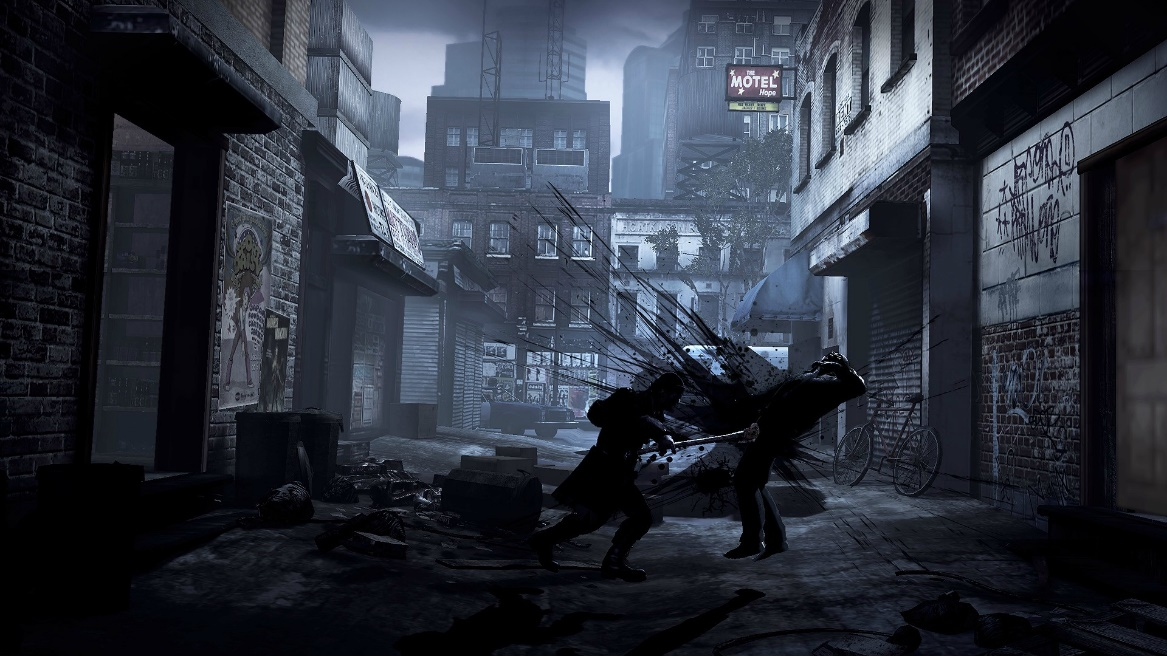
\includegraphics[width=5.30458in,height=2.98414in]{anexos/GDD/GDD-img001.jpg} 
    \caption{Imagen del juego Deadlight. Fuente: http://webvyc.com/deadlight-el-juego-postapocaliptico-de-zombies-del-estudio-espanol-tequila-works/}
    \label{deadlightImage}
    \end{center}
\end{figure}


\section[Men\'us]{\selectlanguage{spanish} Men\'us}
\label{guionTecnico}
\hypertarget{Toc484614215}{}\subsection[Men\'u principal]{\selectlanguage{spanish} Men\'u principal}
\hypertarget{Toc484614216}{}{\selectlanguage{spanish}
Es el men\'u que aparece inmediatamente despu\'es de que se abra el juego y el logo ``Made with Unity'' aparezca. En
este men\'u se pueden acceder a todas las opciones disponibles del juego. La ventana que aparece inicialmente es la que
contiene el t\'itulo ``Da Vinci startup'' y para navegar hacia el resto se debe de arrastrar la pantalla hacia derecha
o izquierda.\ }

{\selectlanguage{spanish}
Si se clica en el bot\'on play que hay en la pantalla inicial se empezar\'a el juego. 


En la siguiente imagen (ver fig. \ref{allMenuImage}) se puede ver un mockup con el conjunto de pantallas del men\'u principal.}


\bigskip

\begin{figure}
    \begin{center}
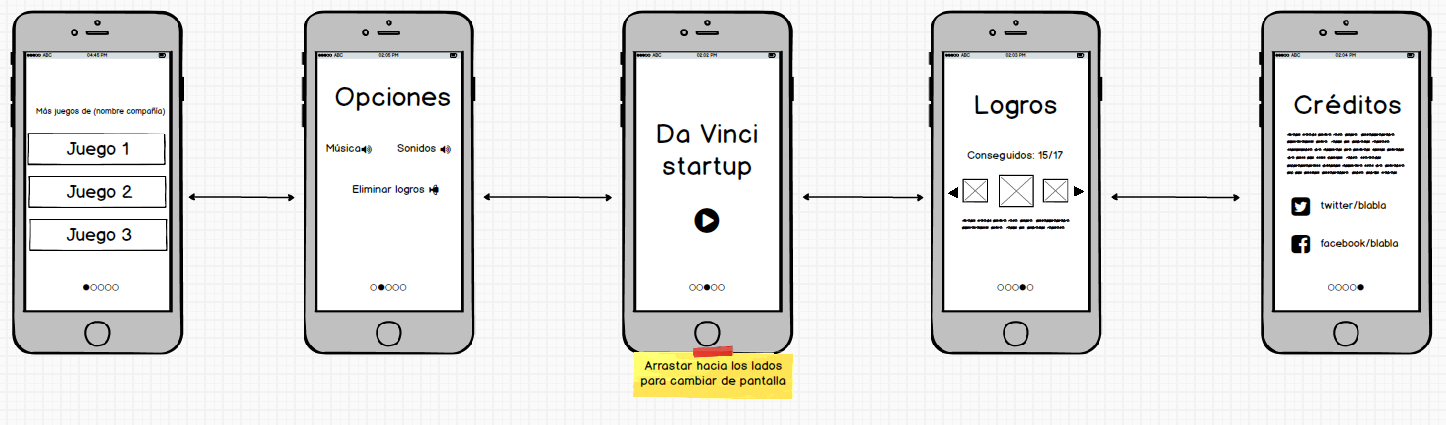
\includegraphics[width=5.90556in,height=1.73542in]{anexos/GDD/GDD-img002.png}
    \caption{Mockup con las pantallas del menú principal. Fuente: elaboración propia}
    \label{allMenuImage}
    \end{center}
    
\end{figure}


\subsection[Logros]{\selectlanguage{spanish} Logros}
\hypertarget{Toc484614217}{}{\selectlanguage{spanish}
Muestra los logros que han sido obtenidos durante el juego. En una l\'inea\ se muestra cu\'antos logros se han
conseguido y el total de los mismos.\ }

{\selectlanguage{spanish}
Bajo esta l\'inea se pueden ver las im\'agenes de los logros junto con un texto descriptivo. Los logros no completados
mostrar\'an su imagen en blanco y negro, mientras que los s\'i completados la mostrar\'an a color.\ }

{\selectlanguage{spanish}
A ambos lados de la\ hilera de im\'agenes se dispondr\'an de sendos botones con forma de flecha que al ser clicados
cambiar\'an el logro que se est\'a seleccionando en ese momento.}

{\selectlanguage{spanish}
El logro seleccionado se muestra con un tama\~no mayor. El texto descriptivo que aparece bajo la hilera de im\'agenes es
el correspondiente al logro seleccionado. En el siguiente mockup (ver fig. \ref{mockupLogros}) se puede ver una representaci\'on visual de dicha pantalla.\ }

\begin{figure}
    \begin{center}
 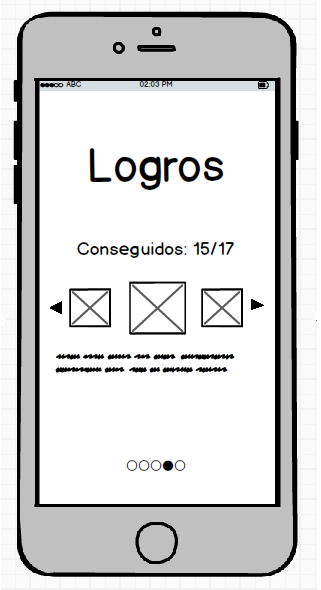
\includegraphics[width=1.35737in,height=2.49485in]{anexos/GDD/GDD-img003.png} 
    \caption{Mockup de la pantalla de logros. Fuente: elaboración propia}
    \label{mockupLogros}
    \end{center}

\end{figure}


\subsection[Cr\'editos]{\selectlanguage{spanish} Cr\'editos}
\hypertarget{Toc484614218}{}{\selectlanguage{spanish}
En un cuadro de texto se da cr\'edito a las personas necesarias: autores de scripts, im\'agenes, m\'usica u otros
elementos utilizados.}

{\selectlanguage{spanish}
Se a\~naden tambi\'en m\'etodos de contacto con el autor. En el siguiente mockup (ver fig. \ref{mockupCreditos}) se puede ver una representaci\'on visual de dicha pantalla.}

\begin{figure}
    \begin{center}
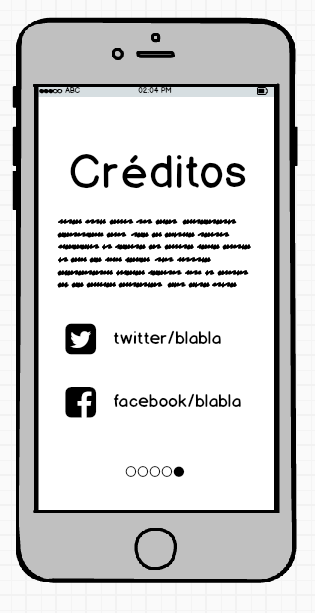
\includegraphics[width=1.30933in,height=2.548in]{anexos/GDD/GDD-img004.png} 
    \caption{Mockup de la pantalla de créditos. Fuente: elaboración propia}
    \label{mockupCreditos}
    \end{center}

\end{figure}


\subsection[Opciones]{\selectlanguage{spanish} Opciones}
\hypertarget{Toc484614219}{}{\selectlanguage{spanish}
En este men\'u (ver fig. \ref{mockupOpciones}) se pueden cambiar diferentes\ aspectos del juegos tales como el volumen de la\ m\'usica o de los efectos
sonoros o\ eliminar los logros obtenidos.}

\begin{figure}
    \begin{center}
 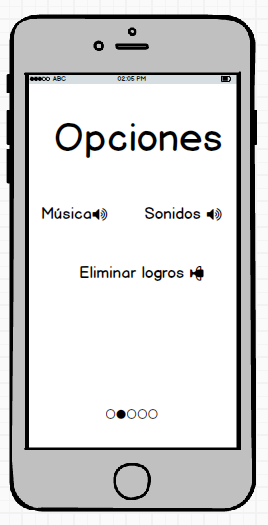
\includegraphics[width=1.3923in,height=2.72745in]{anexos/GDD/GDD-img005.png} 
    \caption{Mockup de la pantalla de opciones. Fuente: elaboración propia}
    \label{mockupOpciones}
    \end{center}

\end{figure}


\subsection[Otros juegos]{\selectlanguage{spanish} Otros juegos}
\hypertarget{Toc484614220}{}{\selectlanguage{spanish}
Men\'u (ver fig. \ref{mockupJuegos}) donde se pueden ver otros juegos creados por el autor. Al clicar en ellos el jugador es redirigido a\ la p\'agina
correspondiente en\ Google Play.}

\begin{figure}
    \begin{center}
 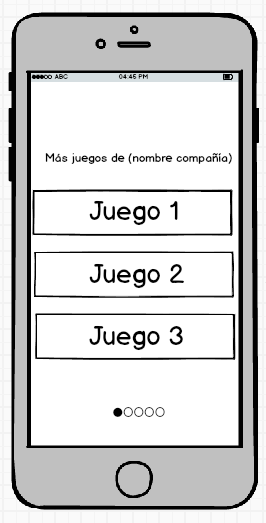
\includegraphics[width=1.38953in,height=2.73205in]{anexos/GDD/GDD-img006.png} 
    \caption{Mockup de la pantalla de otros juegos. Fuente: elaboración propia}
    \label{mockupJuegos}
    \end{center}

\end{figure}


\subsection[Juego]{\selectlanguage{spanish} Juego}
\label{mockupsJuego}
\hypertarget{Toc484614221}{}{\selectlanguage{spanish}
Durante el juego se dispone de una interfaz con\ 3\ botones que\ son el Indicador de personaje, el Indicador de
objetivos y el bot\'on de pausa.}

{\selectlanguage{spanish}
El indicador de personaje muestra una imagen del personaje (de los tres personajes controlables) que controla
actualmente el jugador. Al clicar en el Indicador de personaje este se expande, y al hacerlo se muestran las caras de
los tres personajes controlables. La cara del personaje que el jugador controla en ese momento se mostrar\'a en gris.}

{\selectlanguage{spanish}
Clicando en el icono de alguno de los otros jugadores har\'a que el men\'u se contraiga de nuevo y el personaje
controlado cambie al seleccionado.}

{\selectlanguage{spanish}
El Indicador de objetivos\ muestra el objetivo actual\ que se debe cumplir. Al clicar en el icono del Indicador de
objetivos se muestra una lista desplegable el\ texto descriptivo del objetivo.}

{\selectlanguage{spanish}
Al clicar en el bot\'on de pausa se expandir\'a dicho men\'u mostrando las diferentes opciones que ofrece y se parar\'a
el juego. En el siguiente mockup (ver fig. \ref{mockupJuego}) se puede ver una representaci\'on visual de dicha pantalla.}

\begin{figure}
    \begin{center}
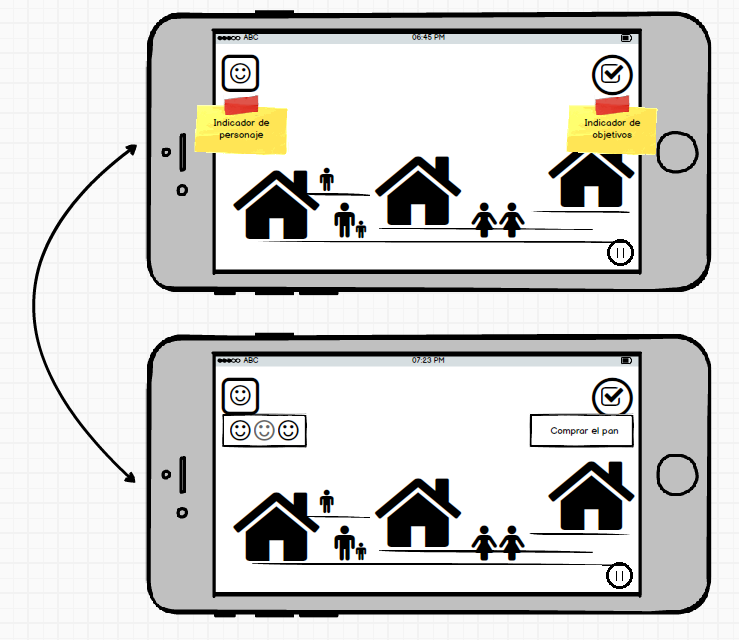
\includegraphics[width=4.08763in,height=3.53967in]{anexos/GDD/GDD-img007.png} 
    \caption{Mockup de la pantalla del juego. Fuente: elaboración propia}
    \label{mockupJuego}
    \end{center}
 
\end{figure}


\subsection[Men\'u conversacional]{\selectlanguage{spanish} Men\'u conversacional}
\hypertarget{Toc484614222}{}{\selectlanguage{spanish}
Este men\'u se abre cuando el jugador interact\'ua con un personaje. La respuesta del personaje\ con el que se est\'a
interactuando\ se muestra en el texto grande, mientras que las posibles respuestas que puede dar el jugador se muestran
en los botones.\ }

{\selectlanguage{spanish}
Cuando se da una respuesta con uno de los botones se actualiza la respuesta del personaje interactuado y\ el texto de
los botones. En el siguiente mockup (ver fig. \ref{mockupConversacion}) se puede ver una representaci\'on visual de dicha pantalla.\ \ }

\begin{figure}
    \begin{center}
 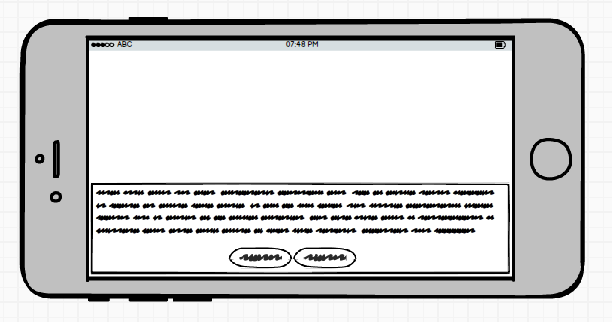
\includegraphics[width=3.36728in,height=1.77154in]{anexos/GDD/GDD-img008.png} 
    \caption{Mockup de la pantalla de conversación. Fuente: elaboración propia}
    \label{mockupConversacion}
    \end{center}

\end{figure}


\subsection[Pausa]{\selectlanguage{spanish} Pausa}
\hypertarget{Toc484614223}{}{\selectlanguage{spanish}
Al clicar\ en el bot\'on de pausa situado en la esquina inferior derecha el juego se pausar\'a. Tambi\'en se abrir\'a un
men\'u desplegable en el que el jugador podr\'a seleccionar entre volver al men\'u principal o abrir el men\'u de
opciones.}

{\selectlanguage{spanish}
Clicando nuevamente en el bot\'on de pausa se cerrar\'a el desplegable y el juego se reactivar\'a. En el siguiente mockup (ver fig. \ref{mockupPausa}) se puede ver una representaci\'on visual de dicha pantalla.}

\begin{figure}
    \begin{center}
 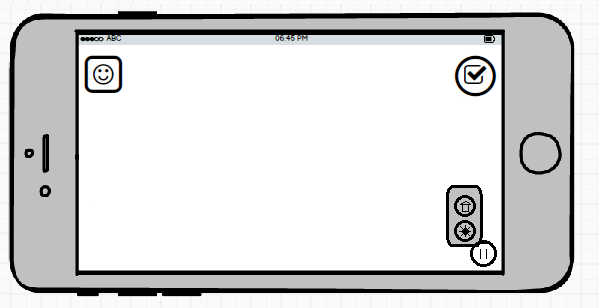
\includegraphics[width=3.36029in,height=1.72756in]{anexos/GDD/GDD-img009.png} 
    \caption{Mockup de la pantalla de pausa. Fuente: elaboración propia}
    \label{mockupPausa}
    \end{center}

\end{figure}


\section[Personajes]{\selectlanguage{spanish} Personajes}
\label{personajes}
\hypertarget{Toc484614224}{}\subsection[Controlables]{\selectlanguage{spanish} Controlables}
\hypertarget{Toc484614225}{}{\selectlanguage{spanish}
Cada uno de los personajes controlables tiene una fortaleza y debilidad en forma de NPCs con los que pueden negociar.
Durante el juego ser\'a necesario controlarlos a todos para poder negociar con los NPCs necesarios para avanzar en la
historia.}

\subsubsection[Leonardo da Vinci]{\selectlanguage{spanish} Leonardo da Vinci}
\hypertarget{Toc484614226}{}{\selectlanguage{spanish}
Protagonista de la historia. Se encarga de dialogar con Andrea del Verrocchio y es el ingeniero del taller. Es respetado
en la Logia de ingenieros por lo que le escuchar\'an cuando vaya. No puede entrar en el puerto y los burgueses no
negocian con \'el.}

\subsubsection[Luca Pacioli]{\selectlanguage{spanish} Luca Pacioli}
\hypertarget{Toc484614227}{}{\selectlanguage{spanish}
Tiene un aspecto desgarbado.\ Es\ uno de los ayudantes de Leonardo durante el juego.\ Puede entrar en el puerto y
negociar con los capitanes y marineros pero no puede negociar con los burgueses\ ni con los ingenieros de\ la Logia.}

\subsubsection[Salai]{\selectlanguage{spanish} Salai}
\hypertarget{Toc484614228}{}{\selectlanguage{spanish}
Luce un\ aspecto elegante. Los burgueses negocian con \'el pero\ no puede entrar en el puerto ni negociar con los
ingenieros de la Logia.}

\subsection[No controlables]{\selectlanguage{spanish} No controlables}
\hypertarget{Toc484614229}{}\subsubsection[Desarrollador]{\selectlanguage{spanish} Desarrollador}
\hypertarget{Toc484614230}{}{\selectlanguage{spanish}
Ataviado con ropas y complementos del siglo XXI aparece en diversos lugares a lo largo del juego. Al hablar con \'el te
pide que punt\'ues la app en Google Play, entre otras cosas.}

\subsubsection[Andrea del Verrocchio]{\selectlanguage{spanish} Andrea del Verrocchio}
\hypertarget{Toc484614231}{}{\selectlanguage{spanish}
Mentor de Leonardo. Da consejos sobre la metodolog\'ia Lean startup. Se encuentra en el taller.}

\subsubsection[Marinero\ portero]{\selectlanguage{spanish} Marinero\ portero}
\hypertarget{Toc484614232}{}{\selectlanguage{spanish}
Se encuentra en la entrada del puerto. Act\'ua como portero, dejando pasar solo a quien considera oportuno.\ Solo
dejar\'a pasar a Luca al puerto.}

\subsubsection[Marinero machaca 1]{\selectlanguage{spanish} Marinero machaca 1}
\hypertarget{Toc484614233}{}{\selectlanguage{spanish}
Puede ser contratado para trabajar en el taller de Leonardo.\ Se encuentra dentro del puerto.}

\subsubsection[Marinero machaca 2]{\selectlanguage{spanish} Marinero machaca 2}
\hypertarget{Toc484614234}{}{\selectlanguage{spanish}
Puede ser contratado para trabajar en el taller de Leonardo. Se encuentra dentro del puerto.}

\subsubsection[Capit\'an 1]{\selectlanguage{spanish} Capit\'an 1}
\hypertarget{Toc484614235}{}{\selectlanguage{spanish}
No quiere comprar el invento pero est\'a ansioso por venderte un barco. Est\'a en el puerto}

\subsubsection[Capit\'an 2]{\selectlanguage{spanish} Capit\'an 2}
\hypertarget{Toc484614236}{}{\selectlanguage{spanish}
No compra el invento pero te cuenta historias fantasiosas\ sobre sus viajes en el mar. Est\'a en el puerto}

\subsubsection[Capit\'an loco]{\selectlanguage{spanish} Capit\'an loco}
\hypertarget{Toc484614237}{}{\selectlanguage{spanish}
Rechaza comprar el invento de Leonardo en primera instancia. Acepta comprarlo despu\'es de que pivote hacia algo que le
interese m\'as (barco propulsado por h\'elice).\ Se encuentra dentro del puerto.}

\subsubsection[Burgu\'es 1]{\selectlanguage{spanish} Burgu\'es 1}
\hypertarget{Toc484614238}{}{\selectlanguage{spanish}
Acepta comprar el producto despu\'es de que lo hagan los capitanes, pero solo si se le a\~nade una gr\'ua para cargar
mercanc\'ias.\ Est\'a en el palacio.}

\subsubsection[Burgu\'es 2]{\selectlanguage{spanish} Burgu\'es 2}
\hypertarget{Toc484614239}{}{\selectlanguage{spanish}
No le interesa el invento pero te vende bonos del estado a un precio baj\'isimo. Est\'a en el palacio.}

\subsubsection[Burgu\'es 3]{\selectlanguage{spanish} Burgu\'es 3}
\hypertarget{Toc484614240}{}{\selectlanguage{spanish}
No le interesa el invento pero te aconseja sobre apuestas deportivas. Est\'a en el palacio.}

\subsubsection[Burgu\'es 4]{\selectlanguage{spanish} Burgu\'es 4}
\hypertarget{Toc484614241}{}{\selectlanguage{spanish}
No le interesa el invento pero te cuenta historias sobre sus a\~nos de gloria cuando era rico. Est\'a en el palacio.}

\subsubsection[Ingeniero 1]{\selectlanguage{spanish} Ingeniero 1}
\hypertarget{Toc484614242}{}{\selectlanguage{spanish}
Es el Gran Maestre.\ }

\subsubsection[Ingeniero 1]{\selectlanguage{spanish} Ingeniero 1}
\hypertarget{Toc484614243}{}{\selectlanguage{spanish}
Es un aprendiz de ingeniero.\ Se unir\'a el equipo de Leonardo si se le pide. Est\'a en la logia.}

\subsubsection[Ingeniero 1]{\selectlanguage{spanish} Ingeniero 1}
\hypertarget{Toc484614244}{}{\selectlanguage{spanish}
Es un ingeniero muy cre\'ido. Solo le interesa hablar de lo muy bueno que es y de los t\'itulos que tiene. Est\'a en la
logia.}

\subsubsection[Ciudadano\ de Florencia 1, 2]{\selectlanguage{spanish} Ciudadano\ de Florencia 1, 2}
\hypertarget{Toc484614245}{}{\selectlanguage{spanish}
Simplemente saluda.\ }

\subsubsection[Ciudadano de Florencia\ 3]{\selectlanguage{spanish} Ciudadano de Florencia\ 3}
\hypertarget{Toc484614246}{}{\selectlanguage{spanish}
Vende opio si le dices la contrase\~na correcta.}

\subsubsection[Ciudadano\ de Florencia 4]{\selectlanguage{spanish} Ciudadano\ de Florencia 4}
\hypertarget{Toc484614247}{}{\selectlanguage{spanish}
Pide dinero}

\subsubsection[Ciudadano\ de Florencia 5]{\selectlanguage{spanish} Ciudadano\ de Florencia 5}
\hypertarget{Toc484614248}{}{\selectlanguage{spanish}
\foreignlanguage{spanish}{Quiere que dones dinero para una asociaci\'on que suena muy falsa.}}

\section[Mec\'anicas de juego]{\selectlanguage{spanish} Mec\'anicas de juego}
\hypertarget{Toc484614249}{}\subsection[Movimiento]{\selectlanguage{spanish} Movimiento}
\hypertarget{Toc484614250}{}{\selectlanguage{spanish}
Los personajes controlables se pueden mover en el plano 2D. Para moverse, se\ toca\ en alg\'un lugar de la pantalla y el
personaje se mover\'a hacia\ la posici\'on tocada\ (solo en el eje x).}

\subsection[Interacci\'on con personajes]{\selectlanguage{spanish} Interacci\'on con personajes}
\hypertarget{Toc484614251}{}{\selectlanguage{spanish}
Al hacer\ tocar en la pantalla\ sobre un personaje el jugador se mover\'a hacia el personaje y al estar a su lado se
abrir\'a el men\'u de conversaci\'on.}

\subsection[Seleccionar personaje]{\selectlanguage{spanish} Seleccionar personaje}
\hypertarget{Toc484614252}{}{\selectlanguage{spanish}
Durante el juego se pueden controlar tres diferentes personajes: Leonardo, Luca y Salai. \ En cualquier momento (siempre
que no se est\'e en una conversaci\'on) se puede cambiar el personaje controlado usando el men\'u
correspondiente.\ Para ello se deber\'a expandir el selector de personaje y clicar en el icono de la cara del personaje
deseado.}

\subsection[Conversar]{\selectlanguage{spanish} Conversar}
\hypertarget{Toc484614253}{}{\selectlanguage{spanish}
Cuando se interact\'ua con un personaje se inicia una conversaci\'on. Para ello se abre autom\'aticamente el men\'u
conversaci\'on, que consiste en: se hace zoom sobre el juego hasta que los cuerpos de ambos personajes quedan en primer
plano;\ se crea una ventana de texto en la parte inferior donde aparece el discurso del personaje que nos est\'e
hablando; debajo del cuadro de texto aparecen botones con las posibles respuestas. Cuando se selecciona una respuesta
se actualiza el cuadro de texto con una contestaci\'on y se actualizan tambi\'en los botones de respuesta.}

\section[Mec\'anicas del mundo]{\selectlanguage{spanish} Mec\'anicas del mundo}
\hypertarget{Toc484614254}{}\subsection[Cambio de escenario]{\selectlanguage{spanish} Cambio de escenario}
\hypertarget{Toc484614255}{}{\selectlanguage{spanish}
Cada escenario tiene puertas que lo conecta con los escenarios adyacentes. Por ejemplo, desde el Taller de Leonardo se
puede acceder a las Calles de Florencia. A su vez desde las Calles de Florencia se puede acceder al puerto. El jugador
solo puede estar en un escenario a la vez, y clicando en las puertas mencionadas anteriormente se cambia de un
escenario a otro y\ se aparece en una posici\'on concreta del escenario (un punto de spawn situado al lado de la
puerta).}

\subsection[Scrolling paralax]{\selectlanguage{spanish} Scrolling paralax}
\hypertarget{Toc484614256}{}{\selectlanguage{spanish}
\foreignlanguage{spanish}{Cuando el jugador se mueve por el mapa el fondo se desplaza tambi\'en de forma horizontal. El
fondo se divide en varias capas, cada una representando un plano a diferente distancia del jugador, y estas se
desplazar\'an a diferente velocidad. Algunas de las capas se sit\'uan entre el jugador y la c\'amara, de forma que
tapan la visi\'on del jugador en ocasiones.}}

\subsection[Completar objetivo]{\selectlanguage{spanish} Completar objetivo}
\hypertarget{Toc484614257}{}{\selectlanguage{spanish}
Tras realizar la acci\'on asociada al objetivo actual, el icono del indicador de objetivo parpadear\'a y variar\'a
ligeramente de tama\~no de forma intermitente. Cuando el jugador abra el men\'u del indicador del objetivo aparecer\'a
un nuevo objetivo y el anterior ser\'a eliminado.}

\section[Escenarios]{\selectlanguage{spanish} Escenarios}
\label{descripcionEscenarios}
\hypertarget{Toc484614258}{}\subsection[Taller de Leonardo]{\selectlanguage{spanish} Taller de Leonardo}
\hypertarget{Toc484614259}{}{\selectlanguage{spanish}
En el taller se puede encontrar a Andrea del Verrocchio, que ser\'a quien dicte los objetivos a cumplir durante la
historia y dar\'a consejos sobre Lean startup.}

{\selectlanguage{spanish}
Conecta con las Calles de Florencia.}

\subsection[Calles de Florencia]{\selectlanguage{spanish} Calles de Florencia}
\hypertarget{Toc484614260}{}{\selectlanguage{spanish}
Las calles de Florencia es el escenario conector en el juego: desde las calles se puede acceder al resto de escenarios
como el taller, el puerto, la logia o el palacio.}

{\selectlanguage{spanish}
Los ciudadanos de Florencia pululan por las calles y\ el jugador podr\'a hablar con ellos.}

\subsection[Palacio de Lorenzo]{\selectlanguage{spanish} Palacio de Lorenzo}
\hypertarget{Toc484614261}{}{\selectlanguage{spanish}
En este edificio se encuentran los burgueses, que solo har\'an negocios con Salai.}

{\selectlanguage{spanish}
Se accede desde las calles de Florencia.}

\subsection[Logia de ingenieros]{\selectlanguage{spanish} Logia de ingenieros}
\hypertarget{Toc484614262}{}{\selectlanguage{spanish}
En este edificio se encuentran los ingenieros, que solo hablar\'an con Leonardo. Se accede desde las calles de
Florencia.}

\subsection[Puerto]{\selectlanguage{spanish} Puerto}
\hypertarget{Toc484614263}{}{\selectlanguage{spanish}
Se encuentran marinos rudos que\ est\'an ociosos. Un marino en la entrada del puerto act\'ua como portero\ dejando
entrar a quien\ considera oportuno. Salai no puede entrar debido a que por su aspecto de clase alta los marineros no le
dejan pasar. Leonardo no puede entrar ya que el puerto es un lugar peligroso y los marineros no le dejan pasar por si
le ocurre algo.}

{\selectlanguage{spanish}
Los marineros pueden ser contratados por Luca para trabajar en el taller.}

\section[Guion\ literario]{\selectlanguage{spanish} Guion\ literario}
\label{guionLiterario}
\hypertarget{Toc484614264}{}{\selectlanguage{spanish}
Solo los ingenieros m\'as sobresalientes son nombrados Gran maestre en la logia de ingenieros de Florencia. Esta es la
ambici\'on de Leonardo da Vinci, el m\'as grande de los ingenieros de Florencia. Ha construido multitud de artefactos
pero todav\'ia tiene un \'ultimo reto por delante antes de pasar de aprendiz a Gran maestre: debe construir un invento
que se venda por un mill\'on de florines.}

{\selectlanguage{spanish}
Leonardo\ est\'a contemplando el vuelo de un p\'ajaro en las calles de Florencia y queda fascinado por la facilidad con
la que la criatura se eleva hacia los cielos. Se le ocurre que si consiguiera construir un artefacto que pudiera hacer
volar a las personas de la misma forma que lo hacen las aves se har\'ia rico\ y se convertir\'ia en un Gran
Maestre.\ Llamar\'a\ a este invento\ {}``el vuelac\'optero''.}

{\selectlanguage{spanish}
Con esta idea en mente va corriendo al taller en el que trabaja junto con su maestro Andrea del Verrochio y sus
aprendices Salai y Luca Paccioli. Una vez all\'i le cuenta la idea a Verrochio y este le promete su ayuda a lo largo de
todo el proceso de construir y comercializar el invento puesto que es un gur\'u de una\ nueva metodolog\'ia de trabajo
inventada en ``Toscana Valley''.\ }

{\selectlanguage{spanish}
Leonardo est\'a ansioso por ponerse manos a la obra\ pero Verrochio le advierte de que para que un proyecto funcione no
se puede trabajar a lo cowboy, hace falta un equipo que aporte los conocimientos que uno no tiene.\ Es necesario
conocer gente, y eso solo se puede hacer saliendo a la calle. En Toscana Valley llaman a esto ``hacer networking''.\ De
esta forma la primera tarea del taller es encontrar a unos obreros que ayuden a construir. Estos obreros ser\'an
marineros parados del puerto, al que solo\ es permitido el acceso a Luca.}

{\selectlanguage{spanish}
Una vez conseguida la mano de obra es necesario conseguir financiaci\'on, para lo cual se pueden tomar diferentes
alternativas que Verrocchio explicar\'a: se puede optar por el bootstrapping o buscar financiaci\'on externa. El taller
deber\'a optar por la segunda opci\'on ya que con el capital que tienen no pueden asumir los costes del proyecto. Para
conseguir financiaci\'on el lugar m\'as adecuado es el palacio donde los burgueses se re\'unen a discutir\ sobre
econom\'ia. Solo Salai, con su estatus de burgu\'es, conseguir\'a que los burgueses le tomen en serio y le proporcionen
los fondos que necesitan.}

{\selectlanguage{spanish}
Conseguidos financiaci\'on y mano de obra, solo falta hacer ingenier\'ia y dise\~nar el producto que se va a construir.
Para ello Leonardo deber\'a convencer a alg\'un ingeniero de la logia para que se una al equipo, y una vez conseguido,
trabajar en los planos.}

{\selectlanguage{spanish}
Leonardo est\'a impaciente, con todos los recursos reunidos solo falta ponerse manos a la obra y construir el
vuelac\'optero. Una vez construido todo el mundo querr\'a uno y se har\'an ricos. Craso error. Verrocchio le quita la
idea r\'apidamente de la cabeza: as\'i no se hacen las cosas en Toscana Valley. Las ideas suenan perfectas en nuestra
cabeza pero rara vez coinciden con las de los\ clientes. As\'i que en lugar de construir el producto y esperar a que
est\'e finalizado para\ venderlo, lo que har\'an ser\'a utilizar un desarrollo iterativo: construir\'an una versi\'on
temprana del vuelac\'optero y le ir\'an a\~nadiendo partes a medida que los clientes digan lo que les gusta y lo que
no.}

{\selectlanguage{spanish}
Pasan unas semanas, la primera iteraci\'on del desarrollo ha sido completada y Leonardo va a hablar con Verrocchio para
preguntar cu\'ales son los siguientes pasos.\ Ahora que tienen un MVP (producto m\'inimo viable) es hora de salir a la
calle y conseguir lo que en Toscana Valley se llama ``early adopters'': gente tan loca como ellos que se atrevan a
comprar un producto novedoso a\'un sin finalizar.}

{\selectlanguage{spanish}
La b\'usqueda es infructuosa y al parecer nadie quiere comprar un vuelac\'optero, pero un capit\'an loco del puerto
sugiere que con ciertos cambios tal vez estar\'ia interesado.}

{\selectlanguage{spanish}
Leonardo le cuenta sobre el desastre a Verrocchio y este le explica que gracias a que no han estado durante meses
gastando dinero y construyendo una versi\'on definitiva del producto, ahora pueden reaccionar a tiempo y cambiar lo que
sea necesario para poder venderlo.}

{\selectlanguage{spanish}
Cuando hay que hacer grandes cambios sobre la hip\'otesis de negocio, se habla de pivotar. De forma que realizando estos
cambios la hip\'otesis de negocio evoluciona de acuerdo a la experiencia adquirida y se acerca m\'as a un modelo de
negocio viable.}

{\selectlanguage{spanish}
De acuerdo a lo requerido por el capit\'an loco, incorporar\'an el vuelac\'optero a un barco para que\ navegue m\'as
deprisa. Una vez construido el nuevo barco se le comunica al capit\'an loco y este lo compra muy gustosamente.}

{\selectlanguage{spanish}
Leonardo le da la noticia a Verrocchio y ambos lo celebran, pero tienen que seguir consiguiendo ventas as\'i que hay que
volver a la calle.\ Al hablar con los burgueses a estos les parece interesante el producto pero no se acomoda del todo
a sus necesidades: lo comprar\'an solo si dispone de una gr\'ua para cargar y descargar mercanc\'ias.}

{\selectlanguage{spanish}
Sabiendo esto, Verrocchio explica que el producto se tiene que adaptar a las necesidades y deseos de los clientes. Esto
se denomina ``customer development''. Los peque\~nos cambios en el modelo de negocio, \ como a\~nadir la gr\'ua al
barco, se denominan pivotar.}

{\selectlanguage{spanish}
Con los nuevos cambios en el barco los burgueses lo compran encantados y Leonardo consigue la meta que ten\'ia que
cumplir para convertirse en Gran maestre. Reflexionando con Verrocchio se da cuenta de c\'omo ha evolucionado la idea
que tuvo originalmente (el vuelac\'optero) hasta convertirse en el barco mercante propulsado por h\'elice. Tambi\'en
piensan en c\'omo habr\'ia resultado todo si no hubieran empleado una metodolog\'ia de desarrollo \'agil y hubieran
empleado muchos esfuerzos en construir el vuelac\'optero antes de mostrarlo a los potenciales clientes.\ }

{\selectlanguage{spanish}
Finalmente Leonardo sale del taller para ir a la logia de ingenieros y la puerta del taller est\'a abarrotada de gente
que quiere comprar uno de sus barcos. La fama de sus veloces barcos mercantes se ha extendido por toda Florencia. En la
logia es convertido en Gran maestre y el ingeniero jefe le explica que la b\'usqueda de su startup ha finalizado. Han
conseguido encontrar su hueco en el mercado y desarrollar su producto. Da Vinci\ startup deja de ser una startup.}

\section[Objetivos]{\selectlanguage{spanish} Objetivos}
\hypertarget{Toc484614265}{}{\selectlanguage{spanish}
El flujo del juego es controlado por el objetivo a cumplir. En todo momento se dispone de un objetivo a cumplir, y al
hacerlo se desbloquea el siguiente y el mundo del juego se actualiza.}

{\selectlanguage{spanish}
De este modo el transcurso del juego se basa en el cumplimiento de los objetivos y son el hilo conductor de la historia.
La lista de los objetivos ordenados por orden de aparici\'on es:}

\liststyleLFOxii
\setcounter{saveenum}{\value{enumi}}
\begin{enumerate}
\setcounter{enumi}{\value{saveenum}}
\item {\selectlanguage{spanish}
Habla con el Gran Maestre}
\item {\selectlanguage{spanish}
Ve al taller y pide ayuda al maestro Verrochio\ \ }
\item {\selectlanguage{spanish}
Ve al puerto y consigue constructores}
\item {\selectlanguage{spanish}
Ve al taller y habla con el maestro Verrochio}
\item {\selectlanguage{spanish}
Consigue financiaci\'on de los burgueses}
\item {\selectlanguage{spanish}
Ve al taller y habla con el maestro Verrocchio}
\item {\selectlanguage{spanish}
Consigue un ingeniero en la logia}
\item {\selectlanguage{spanish}
Ve al taller y habla con el maestro Verrocchio}
\item {\selectlanguage{spanish}
Busca early adopters}
\item {\selectlanguage{spanish}
Ve al taller y cuentale el fracaso al maestro Verrocchio}
\item {\selectlanguage{spanish}
Habla con el capit\'an loco}
\item {\selectlanguage{spanish}
Ve al taller y habla con el maestro Verrocchio}
\item {\selectlanguage{spanish}
Busca m\'as early adopters}
\item {\selectlanguage{spanish}
Ve al taller y habla con el maestro Verrocchio}
\item {\selectlanguage{spanish}
Habla con el burgu\'es}
\item {\selectlanguage{spanish}
Ve al taller y habla con el maestro Verrocchio}
\item {\selectlanguage{spanish}
Habla con el gran maestre}
\end{enumerate}
\section[Logros]{\selectlanguage{spanish} Logros}
\hypertarget{Toc484614266}{}{\selectlanguage{spanish}
Adem\'as de los objetivos se podr\'an desbloquear logros, aunque el desbloqueo de estos no es requerido para completar
el juego. Su funci\'on es meramente coleccionista. Los logros que se podr\'an desbloquear son:}

\liststyleLFOxi
\begin{itemize}
\item {\selectlanguage{spanish}
La ira de los bits caer\'a sobre ti}
\item {\selectlanguage{spanish}
Opio conseguido. Es hora de montar una buena fiesta}
\item {\selectlanguage{spanish}
Has conquistado el coraz\'on de un developer}
\item {\selectlanguage{spanish}
Has completado el primer objetivo}
\item {\selectlanguage{spanish}
Has completado el juego}
\end{itemize}
\section[Assets requeridos]{\selectlanguage{spanish} Assets requeridos}
\hypertarget{Toc484614267}{}\subsection[Modelos 3D]{\selectlanguage{spanish} Modelos 3D}
\hypertarget{Toc484614268}{}\subsubsection[Personajes]{\selectlanguage{spanish} Personajes}
\hypertarget{Toc484614269}{}{\selectlanguage{spanish}
Se necesitar\'a un modelo por cada uno de los personajes del juego. Algunos de ellos reutilizar\'an el mismo modelo
y\ solo\ cambiar\'an las texturas que utilizan.}

{\selectlanguage{spanish}
Los modelos requeridos son:}

\liststyleLFOvi
%\setcounter{saveenum}{\value{enumi}}
\begin{itemize}
%\setcounter{enumi}{\value{saveenum}}
\item {\selectlanguage{spanish}
Leonardo}
\item {\selectlanguage{spanish}
Luca}
\item {\selectlanguage{spanish}
Salai}
\item {\selectlanguage{spanish}
Verrocchio}
\item {\selectlanguage{spanish}
Capit\'an (compartido por los dos capitanes y el capit\'an loco)}
\item {\selectlanguage{spanish}
Marinero (compartido por los dos marineros)}
\item {\selectlanguage{spanish}
Burgu\'es (compartido por todos los burgueses)}
\item {\selectlanguage{spanish}
Ingeniero (compartido por todos los ingenieros)}
\item {\selectlanguage{spanish}
Desarrollador}
\end{itemize}
\subsubsection[Edificios]{\selectlanguage{spanish} Edificios}
\hypertarget{Toc484614270}{}{\selectlanguage{spanish}
Se requerir\'an edificios para todos los escenarios del juego. En algunos de los escenarios (taller, puerto) se
necesitar\'a utiler\'ia que represente el trabajo que ah\'i se hace.}

\subsubsection[M\'usica]{\selectlanguage{spanish} M\'usica}
\hypertarget{Toc484614271}{}{\selectlanguage{spanish}
Se requerir\'a una pista de sonido ambiente por cada uno de los escenarios:}

\liststyleLFOvii
\setcounter{saveenum}{\value{enumi}}
\begin{itemize}
\setcounter{enumi}{\value{saveenum}}
\item {\selectlanguage{spanish}
Taller de Leonardo}
\item {\selectlanguage{spanish}
Logia de ingenieros}
\item {\selectlanguage{spanish}
Calles de Florencia}
\item {\selectlanguage{spanish}
Palacio de Lorenzo}
\item {\selectlanguage{spanish}
Puerto}
\end{itemize}
{\selectlanguage{spanish}
Adem\'as se incluir\'a una pista de sonido para el men\'u principal.}

\subsection[Sprites]{\selectlanguage{spanish} Sprites}
\hypertarget{Toc484614272}{}\subsubsection[IU]{\selectlanguage{spanish} IU}
\hypertarget{Toc484614273}{}{\selectlanguage{spanish}
Durante el juego:}

\liststyleLFOxiii
\begin{itemize}
\item {\selectlanguage{spanish}
Icono selector personajes\ }

\begin{itemize}
\item {\selectlanguage{spanish}
Icono cara Salai}
\item {\selectlanguage{spanish}
Icono cara Luca}
\item {\selectlanguage{spanish}
Icono cara Leonardo}
\end{itemize}
\item {\selectlanguage{spanish}
Icono indicador de objetivos}
\item {\selectlanguage{spanish}
Icono pausa}

\begin{itemize}
\item {\selectlanguage{spanish}
Icono home}
\item {\selectlanguage{spanish}
Icono men\'u opciones}
\end{itemize}
\end{itemize}
{\selectlanguage{spanish}
En el men\'u principal:}

\liststyleLFOxiv
\begin{itemize}
\item {\selectlanguage{spanish}
Fondo de los diferentes men\'us}
\item {\selectlanguage{spanish}
Bot\'on iniciar juego}
\item {\selectlanguage{spanish}
Iconos de logros}
\item {\selectlanguage{spanish}
Flechas de navegaci\'on entre logros}
\item {\selectlanguage{spanish}
Marco para texto de logros}
\item {\selectlanguage{spanish}
Icono Linkedin}
\item {\selectlanguage{spanish}
Iconos altavoces con diferentes vol\'umenes}
\end{itemize}

\bigskip


\bigskip


\bigskip
%\end{document}
